%! Author = gramic
%! Date = 16.04.24

% Preamble
\begin{flushleft}
    \subsection{\gls{local-path-provisioner}}
    \gls{local-path-provisioner} wartet auf einen PVC (Persistence Volume Claim).\\
    Sobald ein Pod existiert, wird auf dem Worker Node ein Volume erzeugt, welches Normalerweise unter dem Pfad \texttt{var/volumes} auf dem Node zu finden ist.\\
    Anschliessend wird ein PV (Pesistence Volume) und dem Volume auf dem Node angefügt.\\
    Anschliessend wird das PV an den PVC gebunden:
    \begin{figure}[H]
        \centering
        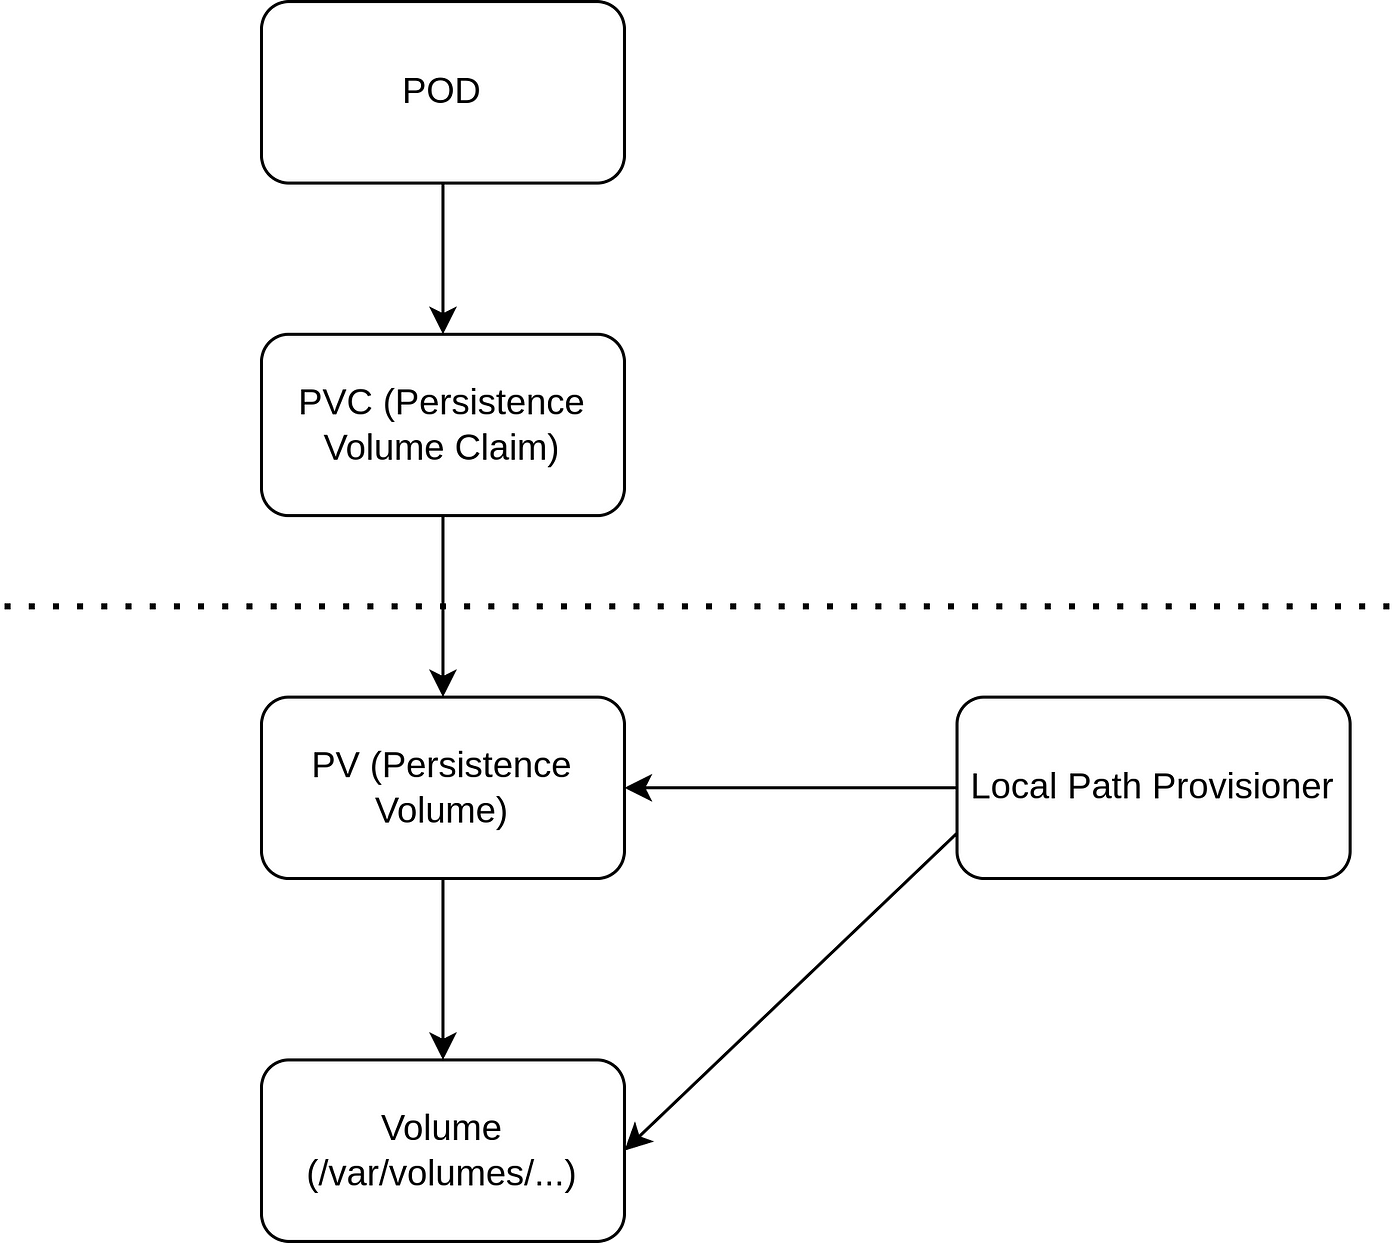
\includegraphics[width=0.75\linewidth]{source/appendix/local-path-provisioner/local-path-provisioner}
        \caption{\gls{local-path-provisioner}\cite{ZTILPG8B}}
        \label{fig:local-path-provisioner}
    \end{figure}
\end{flushleft}